%--------------------------------------------------------------------------------
%\documentclass{article}

\documentclass[a4paper, 12pt]{article}
\usepackage[T1]{fontenc} 
\usepackage[bf]{caption}
\usepackage{hyperref}
\usepackage[all]{hypcap}
\usepackage[utf8]{inputenc}
\usepackage{graphicx}
\usepackage[czech, english]{babel}
\selectlanguage{czech}
\usepackage{subfig}                % \subfloat
\usepackage{color}
\usepackage{url}
\inputencoding{utf8}
%\usepackage[bf]{caption2}
\usepackage{hyperref}
\usepackage[all]{hypcap}
\hypersetup{colorlinks=false, linkbordercolor=1 1 1, citebordercolor=1 1 1}
\usepackage[right]{lineno}
\renewcommand\linenumberfont{\normalfont\tiny\color{blue}}


\title{Jak psat dokumentaci k projektum}
\author{Franta Loginovič <xlogin00@stud.fit.vutbr.cz>}
\date{\today}


%--------------------------------------------------------------------------------


\begin{document}
\selectlanguage{czech}
\maketitle

\section{Úvod}

Tady by mělo být napsané o čem práce je a k čemu to je dobré. Například: Tato práce se zabývá akcelerací
raytracingu na CUDA. Raytracing se používá ve fotorealistické grafice a herní grafice. CUDA umožňuje
akceleraci ...

%%%%%%%%%%%%%%%%%%%%%%%%%%%%%%%%%%%%%%%%%%%%%%%%%%%%%%%%%%%%%%%%%%%%%%%%%%%%%%%%%%%%%%%%

\section{Teorie}

Tady v té kapitole je napsané jak to funguje. Ideálně nějaka ta rovnice, např. \ref{moje-rovnice}. Potom by
tady měla byt uvedena literatura, ze které bylo čerpano, například "Metody sledování paprsku jsou popsané v \cite{Cox2008} \cite{zemcik2006}"


\begin{equation}
  \label{moje-rovnice}
  c = a + b
\end{equation}

Na obrázku \ref{fig:obrazek} je ukázané jak to funguje. Nějaké schémátko pipeline..

\begin{figure}[htb]
  \centering
  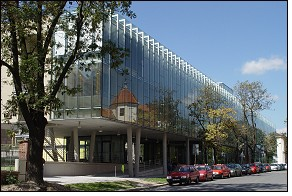
\includegraphics[width=5cm,keepaspectratio]{obrazek.jpg}
  \caption{Nějaký ten diagram, třeba převzaný z \cite{wikipedia}}
  \label{fig:obrazek}
\end{figure}

%%%%%%%%%%%%%%%%%%%%%%%%%%%%%%%%%%%%%%%%%%%%%%%%%%%%%%%%%%%%%%%%%%%%%%%%%%%%%%%%%%%%%%%%

\section{Popis řešení}

Tady stručně popište, jakým způsobem jste prakticky projekt řešili. Uveďte zejména použité
technologie a algoritmy. Zaměřte se hlavně na zajímavé a důležité části implementace a také na
problémy, které jste řešili. Není nutné popisovat každou třídu.

Např. uveďte, jak jste matematický popis z předchozí kapitoly implementovali prakticky.


%%%%%%%%%%%%%%%%%%%%%%%%%%%%%%%%%%%%%%%%%%%%%%%%%%%%%%%%%%%%%%%%%%%%%%%%%%%%%%%%%%%%%%%%

\section{Vyhodnocení}

Tady by mělo být napsané jak to funguje. Protože se jedná o počítačovou grafiku nebo 
vidění, tak by tady měl byt screenshot, ze ktereho bude poznat jak to funguje.
K tomu by měla být idealně tabulka s vyhodnocením jak přesně/rychle to funguje. 

%%%%%%%%%%%%%%%%%%%%%%%%%%%%%%%%%%%%%%%%%%%%%%%%%%%%%%%%%%%%%%%%%%%%%%%%%%%%%%%%%%%%%%%%

\section{Závěr}

Tady by mělo být stručně napsané jak to funguje.


\bibliographystyle{alpha}
\begin{flushleft}
  \bibliography{project}
\end{flushleft}

%\appendix
%\newpage
%\section{}

\end{document}
